% ============================ FINANCE ==================================
\phase{Phase five \textbullet\ Money}{Finance: the plant as a lender sees it}{How the deal is built, why the first design fails, the five moves that rescue it, and the odds that the rescue holds.}\label{sec:finance}

This is the section where we stop being project managers and become what we really are: two finance students asking whether the cash will turn up. We built the plant as a lender would, in a special-purpose company with its own cash-flow waterfall, and then ran it 20,000 times.

\subsection{How the deal is built}
Project finance lends against the project's own cash flows, not against the sponsor's balance sheet \cite{yescombe2014}. That makes every contract around the SPV a piece of risk being handed to whoever can carry it best.

\begin{figure}[H]
\centering
\begin{tikzpicture}[
  spv/.style={rounded corners=3pt,fill=ink,text=paper,font=\small\bfseries,align=center,minimum width=34mm,minimum height=12mm},
  p/.style={rounded corners=2pt,draw=#1,line width=0.7pt,fill=paper,font=\scriptsize,align=center,text width=27mm,inner sep=3pt},
  a/.style={-{Stealth[length=2mm]},line width=0.6pt,color=ink2},
  l/.style={font=\tiny,text=ink2,align=center,fill=paper,inner sep=1pt}]
\node[spv] (s) at (0,0) {Project SPV\\[-1pt]{\scriptsize\normalfont 100 MW hybrid plant}};
\node[p=audit] (spn) at (-5,2.2) {\textbf{Sponsors}\\ 30\% equity, ₹308--440 cr};
\node[p=audit] (len) at (5,2.2) {\textbf{Lenders}\\ 70\% debt, 9\%, 15 yrs};
\node[p=sblue] (epc) at (-5,0) {\textbf{EPC contractor}\\ fixed price, date, delay damages};
\node[p=sblue] (oem) at (-5,-2.2) {\textbf{Electrolyser OEMs}\\ kWh/kg and wear guarantees};
\node[p=sgreen] (off) at (5,0) {\textbf{Refinery}\\ 25-yr fixed price, take-or-pay};
\node[p=sgreen] (ipp) at (5,-2.2) {\textbf{RE sellers}\\ PPAs; firm RE back-up};
\node[p=sochre] (gov) at (0,-2.6) {\textbf{MNRE / CTU}\\ waiver, connectivity, certificate};
\draw[a] (spn) -- node[l,above,sloped]{equity} (s); \draw[a] (len) -- node[l,above,sloped]{loan} (s);
\draw[a] (s) -- node[l,above]{builds} (epc); \draw[a] (oem) -- node[l,above,sloped]{stacks} (s);
\draw[a] (s) -- node[l,above]{hydrogen} (off); \draw[a] (ipp) -- node[l,above,sloped]{power} (s);
\draw[a] (gov) -- (s);
\end{tikzpicture}
\caption{The contract map. Each arrow is a contract that moves a risk off the SPV: construction risk to the EPC contractor, performance risk to the OEMs, price and volume risk to the refinery, resource risk to the power sellers.}
\end{figure}

\noindent The cash waterfall each year is simple to say. Revenue, minus power, operations, insurance and water, gives \textbf{EBITDA}. Minus tax and the maintenance reserve gives \textbf{cash flow available for debt service (CFADS)}. Divide CFADS by that year's interest plus principal and you have the \textbf{debt service cover ratio (DSCR)}, the number every lender watches. Lenders want a minimum near 1.30: thirty paise of spare cash for every rupee owed.

\subsection{What a kilogram costs, by stack}
Our levelised-cost model (Dossier 1's engine, updated) puts the hybrid at \usd{}4.02/kg in the base case and \usd{}4.25 at the median of 100,000 simulations. That is about \usd{}0.19 above a pure alkaline plant: the price of fast ramping and of the AEM option bay. RMI's 2025 India study puts stand-alone on-site projects at \usd{}4.4--4.8/kg \cite{rmi2025}, close to our range. Peer-reviewed work agrees that the electricity price and the load factor drive most of the uncertainty \cite{benalcazar2022,glenk2019}. \confM

\begin{center}\tablefont
\begin{tabularx}{\textwidth}{@{}L c c c c@{}}
\toprule
\thead{Stack, \usd{}/kg of hydrogen} & \thead{Base} & \thead{P10} & \thead{P50} & \thead{P90}\\ \midrule
Alkaline (pressurised) & 3.83 & 3.63 & 4.07 & 4.58\\
\textbf{Hybrid 80/20 (our choice)} & \textbf{4.02} & \textbf{3.79} & \textbf{4.25} & \textbf{4.76}\\
PEM & 5.09 & 4.71 & 5.32 & 5.99\\
AEM & 5.83 & 5.22 & 6.43 & 8.01\\
SOEC & 8.93 & 8.02 & 9.55 & 11.60\\
\bottomrule
\end{tabularx}
\end{center}

\subsection{The first design fails}
At the IOCL price of ₹397/kg, the plant as first costed (\usd{}1,250/kW installed, power at \usd{}38/MWh) does not work.

\begin{center}\tablefont
\begin{tabularx}{\textwidth}{@{}L c c c c@{}}
\toprule
\thead{Measure} & \thead{Base, ₹397} & \thead{Base, ₹279} & \thead{Target, ₹397} & \thead{Target, ₹279}\\ \midrule
Capital cost incl.\ interest during build (₹ cr) & 1,389 & 1,389 & 973 & 973\\
Debt / equity (₹ cr) & 1,028 / 440 & 1,028 / 440 & 718 / 308 & 718 / 308\\
Hydrogen, year 1 (t) & 9,655 & 9,655 & 9,655 & 9,655\\
Revenue, year 1 (₹ cr) & 383 & 269 & 383 & 269\\
Power bill, year 1 (₹ cr) & 182 & 182 & 153 & 153\\
EBITDA, year 1 (₹ cr) & 163 & 49 & 202 & 88\\
Project IRR & 4.3\% & n/a & \textbf{12.2\%} & 1.0\%\\
Equity IRR & $-$0.3\% & n/a & \textbf{18.6\%} & $-$6.0\%\\
Minimum DSCR & 0.63 & $-$0.12 & \textbf{1.36} & 0.45\\
Loan-life cover ratio & 0.87 & 0.04 & 1.63 & 0.65\\
NPV at 10\% (₹ cr) & $-$515 & $-$1,377 & +166 & $-$531\\
\bottomrule
\end{tabularx}
\end{center}

\noindent The power bill alone eats almost half of revenue. The base design cannot repay its loan in any year: a DSCR of 0.63 means the plant earns 63 paise for every rupee of debt service due. To clear a 1.30 cover and a 14\% equity return, it would need \textbf{₹522/kg}, about a third more than any Indian buyer has paid. \confH\ (that the base design fails), \confM\ (for the exact tariff).

\subsection{What you have to believe}
So we ran the problem backwards. Instead of asking ``what does the plant earn?'', we asked ``what price does the plant need, and which moves bring that price down?'' Each bar in the ladder below adds one design-to-cost move to the ones above it.

\begin{figure}[H]
\centering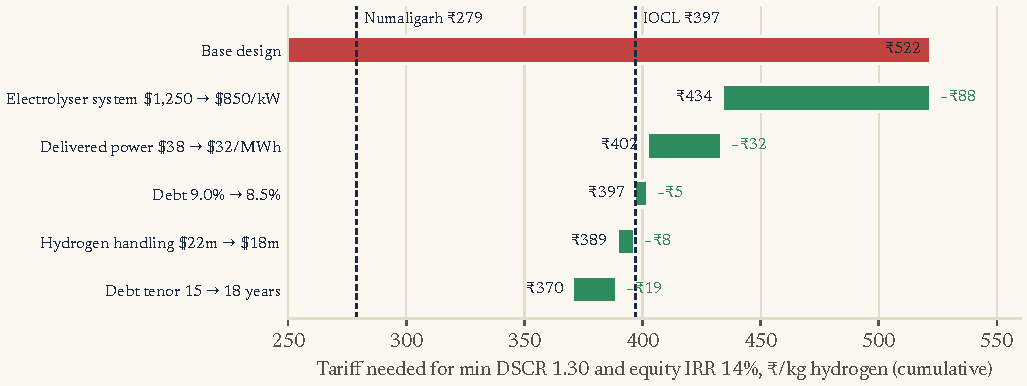
\includegraphics[width=\textwidth]{levers.pdf}
\caption{The lever ladder: required tariff after each cumulative move. Source: \texttt{finance.lever\_ladder()}.}
\end{figure}

\begin{center}\tablefont
\begin{tabularx}{\textwidth}{@{}L c c L@{}}
\toprule
\thead{Move} & \thead{Saves (₹/kg)} & \thead{Needed after} & \thead{Is it believable?}\\ \midrule
Electrolyser system \usd{}1,250 $\rightarrow$ 850/kW & 88 & 434 & Yes, if we buy competitively: Chinese alkaline system prices roughly halved in three years \cite{hfn2025}. The biggest lever by far. \confM\\
Delivered power \usd{}38 $\rightarrow$ 32/MWh & 32 & 402 & Plausible with an oversized solar-wind hybrid and storage near ₹2.86/kWh \cite{sqsolar2025}. \confM\\
Debt 9.0\% $\rightarrow$ 8.5\% & 5 & 397 & Needs a strong sponsor or a green-loan programme. \confM\\
Handling \usd{}22m $\rightarrow$ 18m & 8 & 389 & A shorter pipeline and a smaller buffer. \confM\\
Loan tenor 15 $\rightarrow$ 18 years & 19 & 370 & Common for contracted infrastructure if the buyer is strong. \confM\\
\bottomrule
\end{tabularx}
\end{center}

\begin{finding}[The two numbers that decide everything]
\textbf{The stack price and the power price account for ₹120 of the ₹152/kg gap.} Financing tweaks matter, but they cannot rescue a plant that pays too much for its machines and its electrons. This is the most useful sentence in the book for a procurement team. And note what the ladder cannot reach: Numaligarh's ₹279/kg \cite{rwnrl2026}. Even with every move, it sits ₹91 below what our plant needs. Either that bidder knows something we do not (captive power, very cheap Chinese stacks, a parent willing to accept a low return), or it has under-priced. Section~\ref{sec:paper} asks the same question of the ammonia auctions. \confM
\end{finding}

\subsection{The cover ratio, year by year}
\begin{figure}[H]
\centering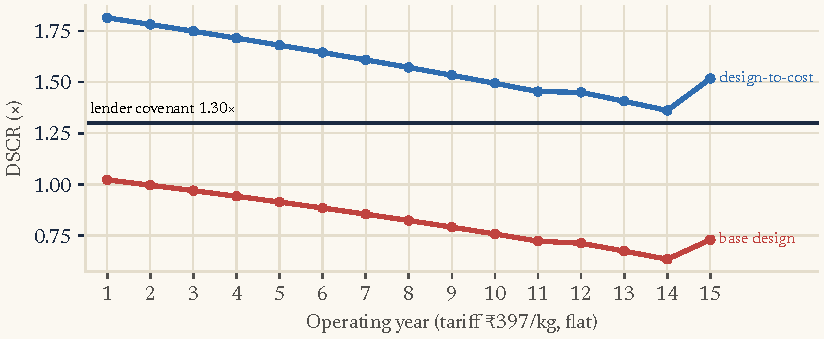
\includegraphics[width=\textwidth]{dscr.pdf}
\caption{DSCR by year at ₹397/kg, base design versus design-to-cost target, 15-year annuity loan. Source: \texttt{finance.py}.}
\end{figure}
The target design starts at 1.81 and slides to 1.36 by year 14. The slide has two causes: stacks wear (more power per kilogram) while the price stays fixed, and operating costs rise 4\% a year while revenue does not. A flat 25-year price with rising costs is a slow squeeze. The jump in year 15 is the alkaline stack swap being absorbed by the reserve built up before it.

\subsection{Twenty thousand futures}
A single base case hides the shape of the risk. We drew every uncertain input from a range (capital cost, power price, load hours, stack efficiency, stack life, interest rate) and added a construction overrun that is skewed upwards, because overruns in large projects are far more common than underruns \cite{flyvbjerg2014}. Our overrun has a median of +5\% and a P80 of +16\%.

\begin{figure}[H]
\centering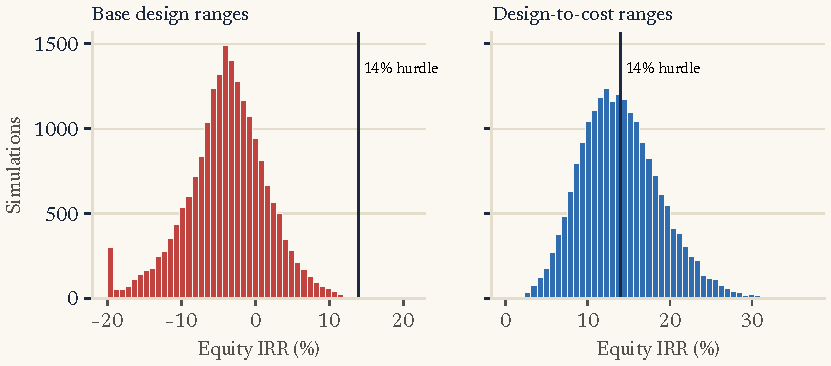
\includegraphics[width=\textwidth]{finance_mc.pdf}
\caption{Equity IRR across 20,000 simulated futures at ₹397/kg. Left: base design ranges. Right: design-to-cost ranges. Source: \texttt{finance.monte\_carlo}.}
\end{figure}

\begin{center}\tablefont
\begin{tabularx}{\textwidth}{@{}L c c c@{}}
\toprule
\thead{At ₹397/kg} & \thead{Base design} & \thead{Target, 15-yr loan} & \thead{Target, 18-yr loan}\\ \midrule
Equity IRR, P10 / P50 / P90 & $-$10.6 / $-$3.7 / 2.9\% & 8.1 / 13.6 / 20.4\% & -- / 14.7\% / --\\
Project IRR, P50 & 2.5\% & 10.4\% & --\\
NPV at 10\%, P50 (₹ cr) & $-$717 & +30 & --\\
Minimum DSCR, P50 & 0.53 & 1.17 & 1.29\\
Chance min DSCR $<$ 1.20 (lock-up) & 99.9\% & \textbf{56.9\%} & \textbf{32.0\%}\\
Chance min DSCR $<$ 1.00 (default risk) & 99.3\% & \textbf{16.3\%} & \textbf{5.4\%}\\
Chance equity IRR $<$ 12\% & 99.8\% & 36.8\% & 30.2\%\\
\bottomrule
\end{tabularx}
\end{center}

\begin{verdict}[Bankable on paper, fragile in practice]
The design-to-cost plant earns 18.6\% for its owners in the base case. But the median of 20,000 futures is 13.6\%, and in more than half of them the cover ratio dips below 1.20 at least once, the level at which lenders typically block dividends. \textbf{The base case is the optimistic case}, because the things that go wrong (overruns, weak wind, early stack wear) are bigger than the things that go right. Stretching the loan to 18 years is the single cheapest fix we found: it cuts the chance of a covenant breach from 57\% to 32\% and of a sub-1.0 year from 16\% to 5\%. \confM
\end{verdict}

\begin{figure}[H]
\centering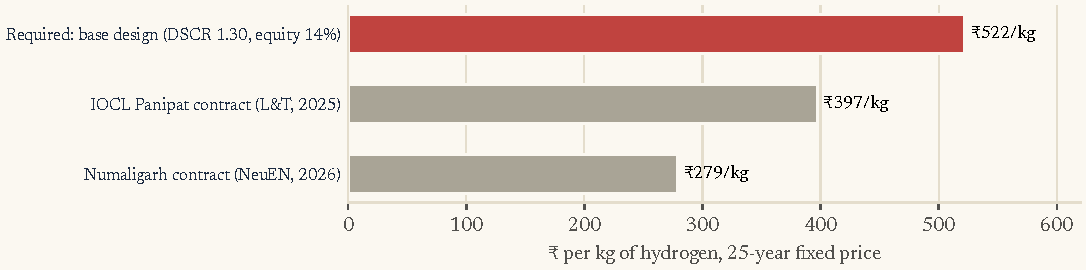
\includegraphics[width=\textwidth]{tariff.pdf}
\caption{What the base design needs against what Indian refineries pay. Sources: \cite{jmkiocl2025,rwnrl2026}; our model.}
\end{figure}

\subsection{What we would ask for at the negotiating table}
Every recommendation below moves a specific risk to someone better able to carry it, and each is tied to a number above.
\begin{enumerate}[leftmargin=1.6em,label={\color{audit}\display\arabic*}]
\item \textbf{An 18-year loan, sculpted to cash flow.} Repayments shaped to fall when stack wear bites, not a flat annuity. (Covenant breach risk 57\% $\rightarrow$ 32\%.)
\item \textbf{Partial indexation of the hydrogen price.} Even 1--2\% a year on the operating-cost share of the price would offset the 4\% cost escalation that drives the DSCR slide.
\item \textbf{Performance guarantees with teeth.} The OEMs guarantee kWh/kg and degradation rate, with damages that cover the extra power. Efficiency is about half our cost; an unguaranteed efficiency is an unhedged power price.
\item \textbf{A fixed-price, date-certain EPC contract} with delay damages at least equal to a month of debt service, and an owner's contingency at P80 (+16\%), not P50.
\item \textbf{Currency and rate hedges.} Imported stacks are priced in dollars or euros; forward cover from order to delivery. An interest-rate swap for the floating part of the debt.
\item \textbf{Reserve accounts.} Six months of debt service in a reserve account (DSRA), plus the major-maintenance reserve already in the model.
\end{enumerate}
\newpage
